\documentclass[12pt]{article}
\usepackage{hpshsetup}
%%%%%%%%%%%%%% 鍵入小論文的題目 %%%%%%%%%%%%%%%%%%%
\newcommand{\TitleName}{111學年度中學生網站小論文比賽文件編譯的另一種選擇}



\begin{document}
\section{前言}
文字文字文字文字,文字文字文字文字。文字文字文字文字,文字文字文字,文字文字文字,文字文字文字文字文字文字文字,文字,文字文字。文字文字文字文字文字,文字文字文字文字文字文字文字,文字文字文字文字,文字文字,文字文字文字文字文字文字文字,文字文字。

文字文字文字文字文字文字,文字文字文字文字文字,文字文字文字文字文字文字,文字文字文字文字文字,文字文字文字文字文字文字文字文字文字文字。文字文字文字文字文字文字:文字文字文字,文字文字文字文字文字,文字文字文字文字文字文字,文字文字文字文字,文字文字文字文字文字。文字文字文字,文字文字文字文字文字文字,文字文字文字文字文字文字文字。文字文字文字文字。文字文字,文字文字文字文字文字文字文字文字,文字文字文字文字文字,文字文字文字文字文字文字,文字文字文字文字文字文字,文字文字文字文字。文字文字文字文字,文字文字文字文字。文字文字文字文字,文字文字文字,文字文字文字,文字文字文字文字文字文字文字,文字,文字文字。文字文字文字文字文字,文字文字文字文字文字文字文字,文字文字文字文字,文字文字,文字文字文字文字文字文字文字,文字文字。

文字文字文字文字文字文字,文字文字文字文字文字,文字文字文字文字文字文字,文字文字文字文字文字,文字文字文字文字文字文字文字文字文字文字。文字文字文字文字文字文字:文字文字文字,文字文字文字文字文字,文字文字文字文字文字文字,文字文字文字文字,文字文字文字文字文字。文字文字文字,文字文字文字文字文字文字,文字文字文字文字文字文字文字。文字文字文字文字。文字文字,文字文字文字文字文字文字文字文字,文字文字文字文字文字,文字文字文字文字文字文字,文字文字文字文字文字文字,文字文字文字文字。



\section{文獻探討}
文字文字文字文字,文字文字文字文字。文字文字文字文字,文字文字文字,文字文字文字,文字文字文字文字文字文字文字,文字,文字文字。文字文字文字文字文字,文字文字文字文字文字文字文字,文字文字文字文字,文字文字,文字文字文字文字文字文字文字,文字文字。

文字文字文字文字文字文字,文字文字文字文字文字,文字文字文字文字文字文字,文字文字文字文字文字,文字文字文字文字文字文字文字文字文字文字。文字文字文字文字文字文字:文字文字文字,文字文字文字文字文字,文字文字文字文字文字文字,文字文字文字文字,文字文字文字文字文字。文字文字文字,文字文字文字文字文字文字,文字文字文字文字文字文字文字。文字文字文字文字。文字文字,文字文字文字文字文字文字文字文字,文字文字文字文字文字,文字文字文字文字文字文字,文字文字文字文字文字文字,文字文字文字文字。

文字文字文字文字文字文字,文字文字文字文字文字,文字文字文字文字文字文字文字文字文字文字文字文字文字,文字文字文字文字,文字文字。文字文字,文字文字文字文字,文字文字文字:文字文字文字文字文字,文字文字文字文字文字,文字文字文字。

文字文字,文字文字文字文字文字,文字文字文字文字文字⋯文字文字文字文字文字文字文字,文字文字文字文字文字,文字文字文字。
文字文字文字文字,文字文字文字文字。文字文字文字文字,文字文字文字,文字文字文字,文字文字文字文字文字文字文字,文字,文字文字。文字文字文字文字文字,文字文字文字文字文字文字文字,文字文字文字文字,文字文字,文字文字文字文字文字文字文字,文字文字。

文字文字文字文字文字文字,文字文字文字文字文字,文字文字文字文字文字文字,文字文字文字文字文字,文字文字文字文字文字文字文字文字文字文字。文字文字文字文字文字文字:文字文字文字,文字文字文字文字文字,文字文字文字文字文字文字,文字文字文字文字,文字文字文字文字文字。文字文字文字,文字文字文字文字文字文字,文字文字文字文字文字文字文字。文字文字文字文字。文字文字,文字文字文字文字文字文字文字文字,文字文字文字文字文字,文字文字文字文字文字文字,文字文字文字文字文字文字,文字文字文字文字。

文字文字文字文字文字文字,文字文字文字文字文字,文字文字文字文字文字文字文字文字文字文字文字文字文字,文字文字文字文字,文字文字。文字文字,文字文字文字文字,文字文字文字:文字文字文字文字文字,文字文字文字文字文字,文字文字文字。

文字文字,文字文字文字文字文字,文字文字文字文字文字⋯文字文字文字文字文字文字文字,文字文字文字文字文字,文字文字文字。




\section{研究方法}

文字文字文字文字文字,文字文字文字。
文字。文字文字文字文字文字,文字文字文字文字文字文字文字,文字文字文字文字,文字文字文字文字文字文字:文字文字文字文字。
文字文字文字文字,文字文字文字,文字文字文字。

\subsection{田野調查及訪視觀察}
文字文字。文字文字文字文字文字文字,文字文字文字,文字文字文字,文字文字文字文字文字,文字文字文字,文字文字文字文字文字。文字文字文字文字,文字文字文字文字。文字文字文字文字文字文字文字文字文字文字文字文字文字文字文字,文字文字文字文字文字文字文字文字文字,文字文字文字文字文字文字文字文字,文字文字文字文字文字。

\subsection{資料歸納}
文字文字文字文字文字文字,文字文字文字文字,文字文字。文字文字文字文字文字文字文字文字文字文字文字⋯文字文字文字文字文字文字,文字文字文字文字文字文字,文字文字文字文字文字文字文字文字文字文字文字。文字文字文字文字:文字文字文字文字文字文字文字,文字文字文字文字文字文字,文字文字文字文字文字⋯文字文字文字,文字文字文字。文字文字文字文字文字文字,文字文字文字文字,文字文字文字文字文字,文字,文字文字。

文字文字文字文字,文字文字文字文字文字,文字文字文字文字文字文字文字,文字,文字文字文字文字。

文字文字文字,文字文字文字文字文字,文字文字文字文字,文字文字⋯文字文字。

文字文字文字文字文字。文字文字文字文字文字,文字文字文字文字文字,文字文字文字文字文字文字,文字,文字文字文字文字文字文字文字,文字文字文字文字文字。文字文字文字,文字文字文字文字文字,文字文字文字文字文字文字文字,文字,文字文字文字文字文字文字。文字文字文字文字文字文字。文字文字。文字文字文字文字,文字文字文字文字文字文字字文字文字文字文字文字,文字文字,文字文字,文字文字文字。文字文字文字文字文字文字文字:文字文字文字文字文字文字。

\subsection{數學表達}
\LaTeX 的數學符號表達方式是一個特色。
在文句中要顯示數學符號可在數學符號前後以 \$ 包圍其中,
例如: \verb|$x^2$| 會被轉換成 $x^2$,
\verb|$x_1$| 會被轉換成 $x_1$。
若要將數學符號單獨成行,
可使用\autocite{einstein}
\begin{equation}
\label{eqn:energy}
E = mc^2 
\end{equation}
\begin{equation}
\sin(\alpha + \beta) = \sin \alpha \cos\beta + \cos \alpha \sin \beta
\end{equation}

\begin{align}
x^\prime  &= \gamma ( x - v t) = \frac{x - vt}{\sqrt{1 - v^2/c^2}} \label{eqn:L1}\\
t^\prime &= \gamma(t - vx/c^2)\label{eqn:L2}
\end{align}
式\ref{eqn:energy} 是 Einstein 有名的質能互換關係式\autocite{yang2006},
式\ref{eqn:L1} 及\ref{eqn:L2} 則是 Lorentz 轉換式\autocite{阮2020}。


文字文字文字文字,文字文字文字文字文字:文字文字文字文字,文字文字文字文字文字文字文字,文字文字文字文字文字,文字文字文字文字?文字文字文字文字文字文字,文字文字文字,文字文字文字文字,文字文字文字文字文字文字:文字文字文字文字文字文字,文字文字文字文字。文字文字文字文字文字文字,文字文字文字文字,文字文字文字文字文字文字文字,文字文字文字文字文字文字。文字文字文字文字。文字文字文字文字文字,文字文字,文字文字文字,文字文字文字,文字文字字文字。



\section{研究分析與結果}


文字文字。文字文字文字文字文字文字,文字文字文字,文字文字文字,文字文字文字文字文字,文字文字文字,文字文字文字文字文字。文字文字文字文字,文字文字文字文字。文字文字文字文字文字文字文字文字文字文字文字文字文字文字文字,文字文字文字文字文字文字字文字文字,文字文字文字文字文字文字文字文字,文字文字文字文字文字。

文字文字文字文字文字文字,文字文字文字文字,文字文字。文字文字文字文字文字文字文字文字文字文字文字文字文字文字文字文字文字,文字文字文字文字文字文字,文字文字文字文字文字文字文字文字文字文字文字。文字文字文字文字文字文字文字文字文字文字文字,文字文字文字文字文字文字,文字文字文字文字文字文字文字文字,文字文字文字。文字文字文字文字文字文字,文字文字文字文字,文字文字文字文字文字,文字,文字文字。

\bxfigure[!htp]{模擬波動在粗細介質不同的繩子上傳遞的過程。
粗細兩段繩子是串聯並且兩端點為固定端,
波動經兩界面時會有部份穿透、部份反射,
經過交會重疊後的波形。\label{fig:rope}}
{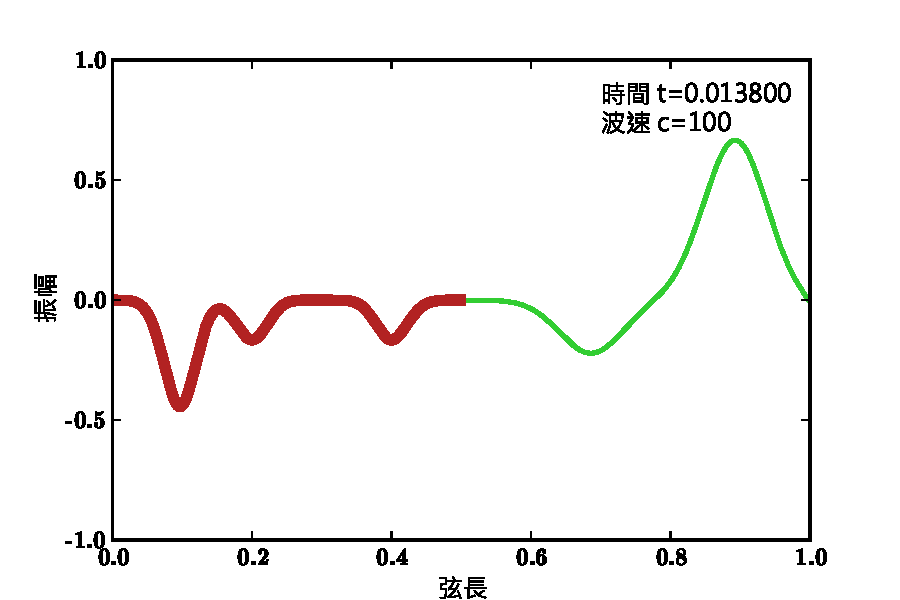
\includegraphics[width=.6\linewidth]{wave_inhomo_0276}}
{圖片來源:免費圖片\autocite{unsplash}}


文字文字文字文字文字。見圖\ref{fig:rope}文字文字文字文字文字,文字文字文字文字文字,文字文字文字文字文字文字,文字,文字文字文字文字文字文字文字,文字文字文字文字文字。文字文字文字,文字文字文字文字文字,文字文字文字文字文字文字文字,文字,文字文字文字文字文字文字。文字文字文字文字文字文字。文字文字。文字文字文字文字,文字文字文字文字文字文字字文字文字文字文字,文字文字,文字文字,文字文字文字。文字文字文字文字文字文字文字:文字文字文字文字文字文字。

文字文字文字文字,文字文字文字文字文字:文字文字文字文字,文字文字文字文字文字文字文字,文字文字文字文字文字,文字文字文字文字?文字文字文字文字文字文字,文字文字文字,文字文字文字文字,文字文字文字文字文字文字:文字文字文字文字文字文字,文字文字文字文字。文字文字文字文字文字文字,文字文字文字文字,文字文字文字文字:文字字文字,文字文字文字文字文字文字。文字文字文字文字。文字文字文字文字文字,文字文字,文字文字文字,文字文字文字,文字文字文字文字。文字文字。文字文字文字文字文字文字,文字文字文字,文字文字文字,文字文字文字文字文字,文字文字文字,文字文字文字文字文字。文字文字文字文字,文字文字文字文字。文字文字文字文字文字文字文字文字文字文字文字文字文字文字文字,文字文字文字文字文字文字字文字文字,文字文字文字文字文字文字文字文字,文字文字文字文字文字\autocite{阮2020}。

文字文字文字文字文字文字,文字文字文字文字,文字文字。文字文字文字文字文字文字文字文字文字文字文字文字文字文字文字文字文字,文字文字文字文字文字文字,文字文字文字文字文字文字文字文字文字文字文字。文字文字文字文字文字文字文字文字文字文字文字,文字文字文字文字文字文字,文字文字文字文字文字文字文字文字,文字文字文字。文字文字文字文字文字文字,文字文字文字文字,文字文字文字文字文字,文字,文字文字。


文字文字文字文字文字。文字文字文字文字文字,文字文字文字文字文字,文字文字文字文字文字文字,文字,文字文字文字文字文字文字文字,文字文字文字文字文字。文字文字文字,文字文字文字文字文字,文字文字文字文字文字文字文字,文字,文字文字文字文字文字文字。文字文字文字文字文字文字。文字文字。文字文字文字文字,文字文字文字文字文字文字字文字文字文字文字,文字文字,文字文字,文字文字文字。文字文字文字文字文字文字文字:文字文字文字文字文字文字。

文字文字文字文字,文字文字文字文字文字:文字文字文字文字,文字文字文字文字文字文字文字,文字文字文字文字文字,文字文字文字文字?文字文字文字文字文字文字,文字文字文字,文字文字文字文字,文字文字文字文字文字文字:文字文字文字文字文字文字,文字文字文字文字。文字文字文字文字文字文字,文字文字文字文字,文字文字文字文字:文字字文字,文字文字文字文字文字文字。文字文字文字文字。文字文字文字文字文字,文字文字,文字文字文字,文字文字文字,文字文字文字文字。

\section{研究結論與建議}

文字文字文字文字文字,文字文字文字。
文字。文字文字文字文字文字,文字文字文字文字文字文字文字,文字文字文字文字,文字文字文字文字文字文字:文字文字文字文字。
文字文字文字文字,文字文字文字,文字文字文字。

文字文字。文字文字文字文字文字文字,文字文字文字,文字文字文字,文字文字文字文字文字,文字文字文字,文字文字文字文字文字。文字文字文字文字,文字文字文字文字。文字文字文字文字文字文字文字文字文字文字文字文字文字文字文字,文字文字文字文字文字文字字文字,文字文字文字文字文字文字文字文字,文字文字文字文字文字。

文字文字文字文字文字文字,文字文字文字文字,文字文字。文字文字文字文字文字文字文字文字文字文字文字文字文字文字文字文字文字,文字文字文字文字文字文字,文字文字文字文字文字文字文字文字文字文字文字。文字文字文字文字:文字文字文字文字文字文字文字,文字文字文字文字文字文字,文字文字文字文字文字文字文字文字,文字文字文字。文字文字文字文字文字文字,文字文字文字文字,文字文字文字文字文字,文字,文字文字。

\bxfigure[!htp]{水波槽兩個點波源同相振動干涉圖樣,
可明顯看出有7條節線。\label{fig:tank}}
{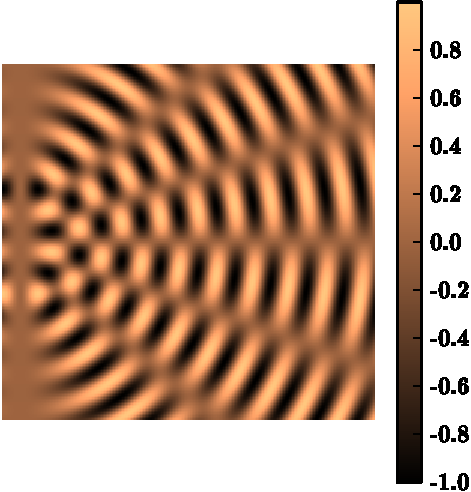
\includegraphics[width=.4\linewidth]{watertank}}
{圖片來源:免費圖片\autocite{unsplash}}

文字文字文字文字文字。文字文字文字文字文字,文字文字文字文字文字,文字文字文字文字文字文字,文字,文字文字文字文字文字文字文字,文字文字文字文字文字。文字文字文字,文字文字文字文字文字,文字文字文字文字文字文字文字,文字,文字文字文字文字文字文字。文字文字文字文字文字文字。文字文字。文字文字文字文字,文字文字文字文字文字文文字文字文字文字文字,文字文字,文字文字,文字文字文字。文字文字文字文字文字文字文字:文字文字文字文字文字文字。文字文字。文字文字文字文字文字文字,文字文字文字,文字文字文字,文字文字文字文字文字,文字文字文字,文字文字文字文字文字。文字文字文字文字,文字文字文字文字。文字文字文字文字文字文字文字文字文字文字文字文字文字文字文字,文字文字文字文字文字文字字文字文字,文字文字文字文字文字文字文字文字,文字文字文字文字文字。

\bxfigure[!htp]{母與子。\label{fig:kater}}
{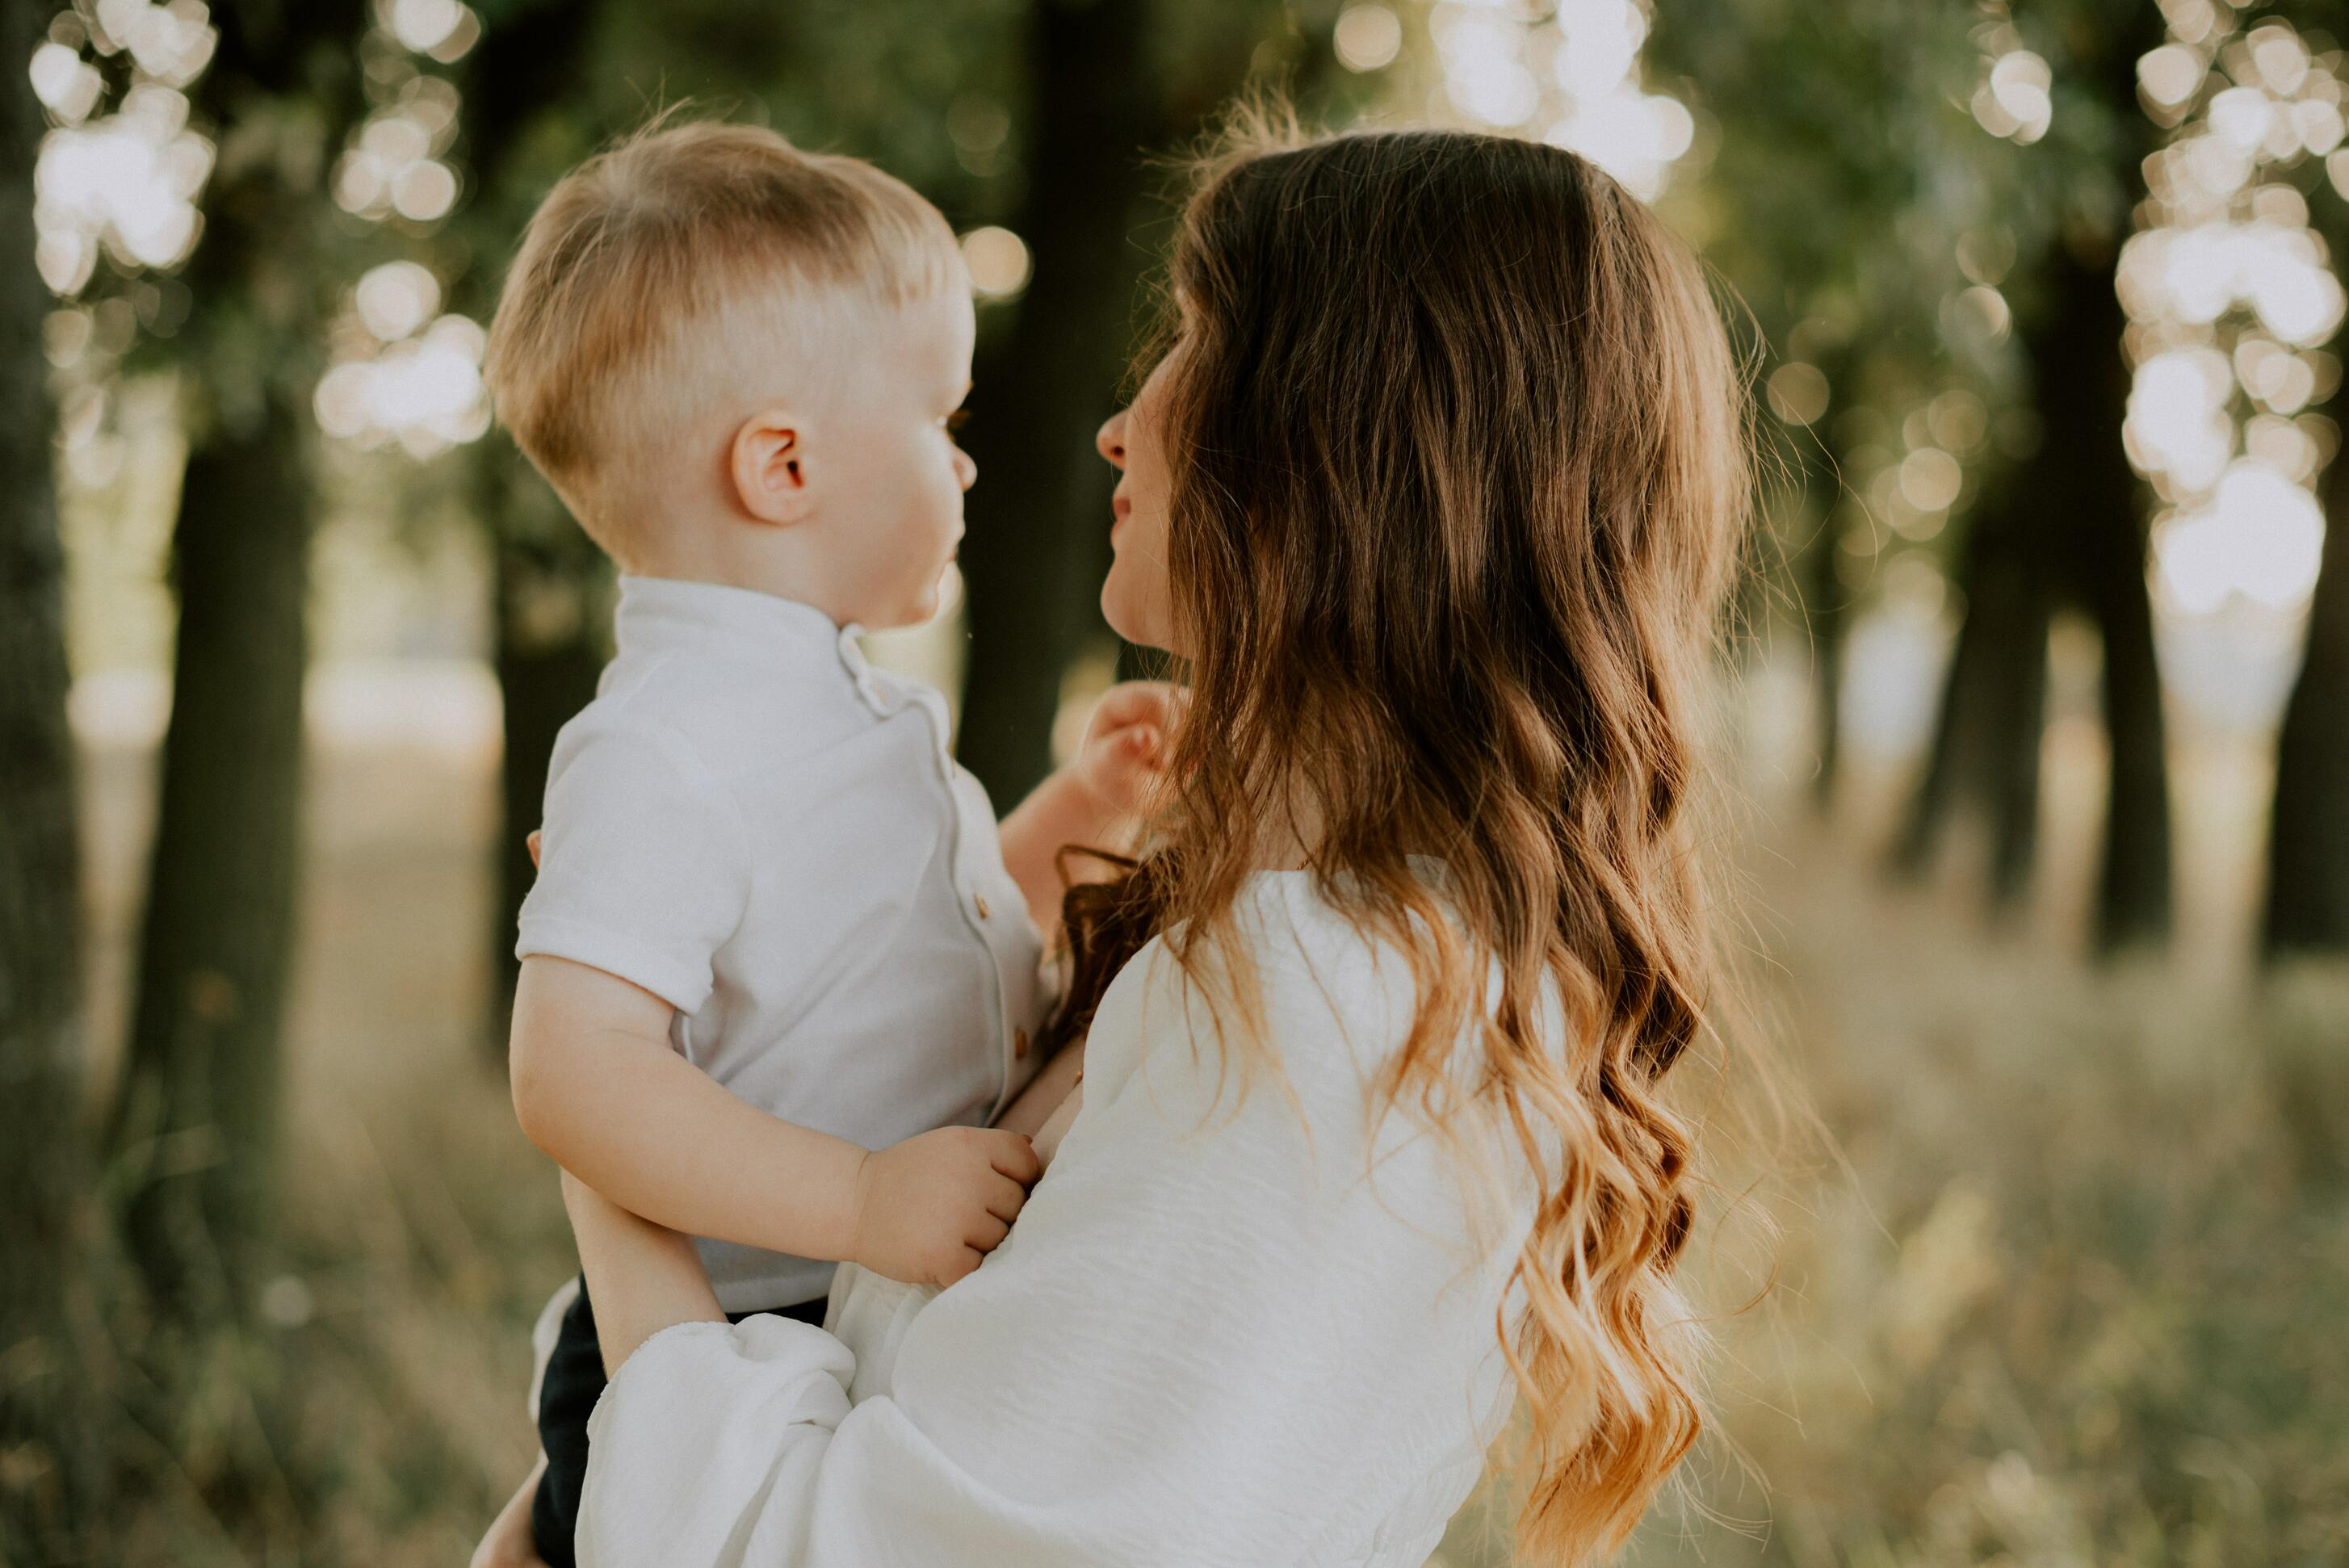
\includegraphics[width=.5\linewidth]{katerREDU.jpg}}
{圖片來源:免費圖片\autocite{unsplash}}

文字文字文字文字文字文字,文字文字文字文字,文字文字。文字文字文字文字文字文字文字文字文字文字文字文字文字文字文字文字文字,文字文字文字文字文字文字,文字文字文字文字文字文字文字文字文字文字文字。文字文字文字文字文字文字文字文字文字文字文字,文字文字文字文字文字文字,文字文字文字文字文字文字文字文字,文字文字文字。文字文字文字文字文字文字,文字文字文字文字,文字文字文字文字文字,文字,文字文字。


文字文字文字文字文字。\textcite{fowles}提到\textbf{「文字文字文字文字文字,文字文字文字文字文字,文字文字文字文字文字文字」},文字,文字文字文字文字文字文字文字,文字文字文字文字文字。文字文字文字,文字文字文字文字文字,文字文字文字文字文字文字文字,文字,文字文字文字文字文字文字。文字文字文字文字文字文字。文字文字。文字文字文字文字,文字文字文字文字文字文字字文字文字文字文字,文字文字,文字文字,文字文字文字。文字文字文字文字文字文字文字:文字文字文字文字文字文字。

文字文字文字文字,文字文字文字文字文字:文字文字文字文字,文字文字文字文字文字文字文字,文字文字文字文字文字,文字文字文字文字?文字文字文字文字文字文字,文字文字文字,文字文字文字文字,文字文字文字文字文字文字:文字文字文字文字文字文字,文字文字文字文字。文字文字文字文字文字文字,文字文字文字文字,文字文字文字文字:文字字文字,文字文字文字文字文字文字。文字文字文字文字。文字文字文字文字文字,文字文字,文字文字文字,文字文字文字,文字文字文字文字\cite{ter1971}。


\bxtable[!htp]{和平高中一月份文具使用量\label{tbl:pen}}
{
\begin{tabular}{cccrr}
\toprule
項次 & 名稱 & 數量 & 單價 & 總價 \\
\midrule
1 & 鉛筆  & 12 & 2.0 & 24.0 \\
2 & 鋼筆 & 3 & 100.0& 300.0 \\
3 & 膠水 & 5 & 10.0 & 50.0 \\
4 & 白報紙 & 30 & 100 & 3000.0\\
\bottomrule
\end{tabular}}
{資料來源:和平高中總務處}



文字文字文字文字,文字文字文字文字文字:文字文字文字文字,文字文字文字文字文字文字文字,文字文字文字文字文字,文字文字文字文字?文字文字文字文字文字文字,文字文字文字,文字文字文字文字,文字文字文字文字文字文字:文字文字文字文字文字文字,文字文字文字文字。文字文字文字文字文字文字,文字文字文字文字,文字文字文字文字:文字字文字,文字文字文字文字文字文字。文字文字文字文字。文字文字文字文字文字,文字文字,文字文字文字,文字文字文字,文字文文字文字\autocite{dirac}。




%\renewcommand{\refname}{參、參考文獻}

\printbibliography[title={陸、參考資料}]
%\printbibliography[keyword=zh, title={肆、參考文獻}]
%\printbibliography[notkeyword=zh, heading=none]


\end{document}
